\chapter{Guidance Assessment Conditions}\label{Ch:AssessmentConditions}

%Also talk about algorithm parameters used to generate trajectories
\section{Entry Conditions and Targets}
The entry guidance strategy is assessed for an MSL-class vehicle with mass $m = 2804$ kg, and area $S = 15.8\, \mathrm{m}^2$. The entry state and associated standard deviations at the entry interface are given in Table~\ref{Table:StateEntryInterface}. By assumption, altitude determines the entry interface point, and thus $\sigma_h = 0$. Given the mean and standard deviation of the entry interface state, a specified prebank angle, and a chosen $v_0$ at which phase 2 guidance begins, the mean and covariance of the state at $v_0$ are determined by integrating Eq.~\eqref{Eq:dynamics:altitude:time}-\eqref{Eq:dynamics:fpa:time} until $v<v_0$. We assume that the distribution remains approximately normal. In practice this appears to be true; the limited aerodynamic nonlinearities at high altitudes do not cause significant changes to the distribution. Note that the parametric uncertainties are also included in determining the mean and covariance at $v_0$.

The resulting mean state and deviations at the start of closed-loop guidance are given in Table~\ref{Table:StateRangeControl}. These are the values used in the solution of the optimal control process. Note that we set $s(v_0) = 0$ for simplicity of discussion, but the total range from the entry interface to the target is 223 km + the optimal range of the solution to the ROGP. 
Similar to the altitude at the entry interface, after propagation to a fixed velocity, $\sigma_v = 0$. The 3$\sigma$ uncertainty in the ballistic coefficient and lift-to-drag ratio is $15\%$. Atmospheric density uncertainty is modeled with the symmetrized Mars Climate Database profile in Fig.~\ref{Fig:DensityVariations}, with the boundary interpreted as the 3$\sigma$ value.
%TODO: Double check these tables, esp EI state. Compare to Guangfei, maybe est with UT in time domain?
\begin{table}[h!]
	\centering
	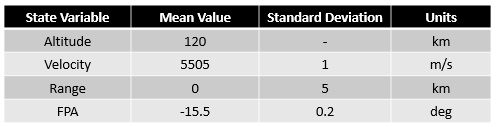
\includegraphics[width=0.85\textwidth]{Images/EntryInterfaceState}
	\caption{The mean state and standard deviations at the entry interface.}
	\label{Table:StateEntryInterface}
\end{table}
\begin{table}[h!]
	\centering
	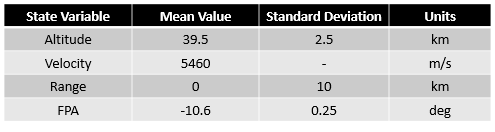
\includegraphics[width=0.85\textwidth]{Images/OptimizationState}
	\caption{The mean state and standard deviations at the start of closed-loop guidance.}
	\label{Table:StateRangeControl}
\end{table}

\section{Robust Optimal Control Solution Parameters}
\begin{table}[h!]
	\centering
	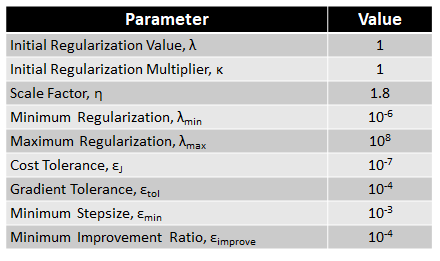
\includegraphics[width=0.75\textwidth]{Images/DDP_Parameters}
	\caption{Algorithm parameters used in all numerical results.}
	\label{Table:DDPParameters}
\end{table}
Table~\ref{Table:DDPParameters} summarizes the algorithm parameters governing the linesearch, regularization, and stopping conditions. 
The smooth saturation approximation uses $M = 20$. The trajectory is discretized into $ N=250 $ velocity steps, with four Euler integration steps per velocity step. The value of $ N $ and the number of integration steps were chosen by validating the terminal altitude and downrange distance against adaptive stepsize integration using MATLAB's \textit{ode45} function. The acceptable error tolerance across all sigma points was 100 m.

\begin{figure}[h!]
	\centering
	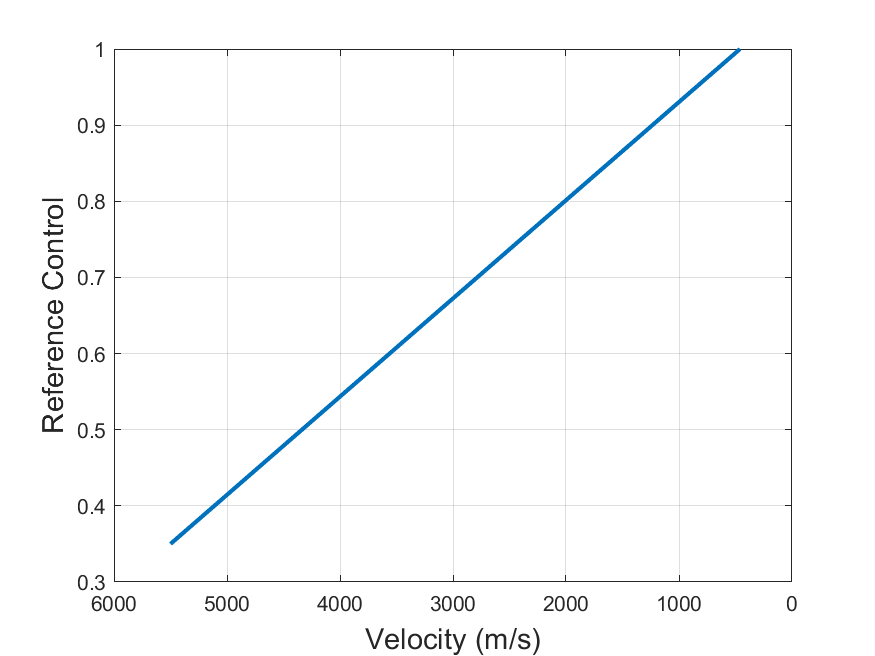
\includegraphics[width=0.75\textwidth]{Images/GuessControl}
	\caption{The reference control used to initialize DDP.}
	\label{Fig:GuessControl}
\end{figure}
%Guess trajectory, show it and discuss. 
A trajectory-control pair is required to initialize the DDP algorithm. In all numerical examples, the initial guess at the optimal reference control is the linear ramp depicted in Fig~\ref{Fig:GuessControl}. This guess is motivated by experience with altitude optimal trajectories, which feature a minimum lift arc followed by a full lift up arc. Such a control has zero margin (in one direction) at every velocity. Our choice is motivated by a similar progression from lift down to lift up, but more gradual and with significant margin throughout. We remark that the solutions are not sensitive to the initial guess. A numerical demonstration is given in Section~\ref{Sec:ConvergenceProperties}.

All solutions consider static gains. In the first section we consider two sets of gains, $K_1=[0,0,0]$ and $K_2 = [0.13,-0.04,-2.5]$, to highlight the impact of the reference trajectory. $K_2$ was chosen to provide to minimize the UT-estimated value of $\sigma_s$ for the initial reference control. Later results use jointly optimized gains. For these cases, the initial guess at the optimal gains is $K_2$. In all examples, unless otherwise noted, the DDP algorithm is applied with the simplification proposed in Subsection~\ref{Sec:DDP_Simplification}.

\subsection{Selecting the UT Parameter}
%Show results for a fixed profile sweeping alpha and show that the estimates are monotonic wrt to the parameter. As result, there exists an alpha that minimizes the error in altitude and range, generally not the same alpha. 

Our earlier example in Section~\ref{Subsec:UQExample} showed that proper selection of $\alpha$ is important, especially for the range variable. In the numerical assessments presented in the Chapter~\ref{Ch:NumericalAssessment}, we consider weight combinations on the grid $w_h\times w_s = [0,3]\times[0,3]$. As such, we selected $\alpha$ to minimize the UT-estimation error in $\sigma_s$ for the optimal solution with $w_h=w_s=1.5$, i.e., at the center point of the grid. We considered integer values of $\alpha$ between 6 and 20, and solved the ROGP for each value. A Monte Carlo simulation was performed for each $\alpha$ and the optimal choice was $\alpha=15$. 
%Note that it is a coincidence that the $\alpha$ in the example of Subsection~\ref{Subsec:UQExample} was the same value. 
% Thinking along the lines, that, minimizing error at the center might keep the error low (enough) at the other points.

\section{Simulation}
%Primary metrics include the 3$\sigma$ low altitude and the 3$\sigma$ range error at the terminal velocity. Some discussion of the mean altitude and range as well. 
Unless otherwise noted, each Monte Carlo simulation is conducted with 3000 sample trajectories. The samples are drawn using Latin Hypercube sampling. The equations of motion are simulated in the time domain, and the bank angle command is updated at a rate of 1 Hz. The bank angle magnitude is subject to the same limits applied during optimization, $0^{\circ}\le|\sigma|\le90^{\circ}$, and the magnitude of the bank angle rate is limited to $20^{\circ}/s$. No bank angle acceleration limit is applied. Range error is the distance between the terminal downrange distance defined by the reference trajectory and the downrange distance flown. The primary metrics we will examine are the 3$\sigma$-low altitude $=\bar{h}-3\sigma_h$ and 3$\sigma$ range error $= 3\sigma_s$ at the final velocity, $v_f=460$m/s. The terminal state distributions are generally non-Gaussian, and in practice percentiles are often used to specify mission requirements. However, metrics based on the mean and standard deviation are presented, because these are the values estimated by the unscented transform, which allows for a direct comparison with the Monte Carlo results.

%WHile simplifcation of models, like the atm density model, introduce conservatism. We simulate using the same models to allow a direct comparison. 

%%% Local Variables: ***
%%% mode: latex ***
%%% TeX-master: "thesis.tex" ***
%%% End: ***
